\chapter{String Theory and M-Theory}

This lecture is organized around a remarkably sharp idea. We want to understand, first, why gravity is built into string theory and, second, why string theory is so much more tightly constrained than the mechanics of point particles. The guiding principle is not elegance for its own sake. It is consistency: if we refine the description of a propagating string by adding more and more of its microscopic structure, do the answers settle down to a definite limit? These notes follow Leonard Susskind's lecture closely and are prepared from source material credited to Leonard Susskind, LazyingArt LLC, and Video2Book.

\section{Consistency First: From Particles to Strings}

Susskind begins with the ordinary mechanics of particles on curved spaces in order to calibrate our expectations. A point particle can move on a smooth curved surface without any difficulty. Classically it moves on a geodesic, that is, on the straightest possible path intrinsic to the surface. Quantum mechanically one may ask for amplitudes rather than trajectories, but the same basic question remains: when we define the theory by breaking time evolution into many tiny steps and then letting the steps become finer and finer, do we get a sensible limit?

For an ordinary particle the answer is yes. In classical mechanics the motion is governed by differential equations whose solutions are smooth when the geometry is smooth. In quantum mechanics the corresponding problem is controlled by the Schr\"odinger equation, or equivalently by the path integral, and again the continuum limit exists. So curved-space particle mechanics is a perfectly good theory.

\subsection{Question \& Answer}

\paragraph{Question.} What does it mean for the continuum limit to exist?

\paragraph{Answer.} It means that after we discretize the motion and then refine the discretization, the physical quantities we compute stabilize. The trajectory, the propagator, the energy spectrum, or any other observable should approach a definite answer instead of drifting as more short-distance detail is included. For point particles on smooth spaces that is exactly what happens.

Now comes the contrast. String theory is about extended objects, not points. A string is not specified by a position and a velocity alone; it carries infinitely many vibrational degrees of freedom. Once that is true, the question of existence of the limit becomes far subtler. To see the issue with the fewest moving parts, Susskind places the string on the simplest curved target space he can draw: a sphere.

\section{A Point Particle on a Sphere}

Before we place a string on the sphere, we do the point-particle problem carefully. The target space is a sphere of radius \(r\). On the board the radius is labeled by \(R\); in the formulas below we keep the lecture's spoken notation \(r\).

\begin{figure}[h]
\centering

\includegraphics[width=0.56\textwidth]{lecture_09_figure_02.png}
\caption{Sphere sketch with radius label.}
\end{figure}

\begin{figure}[h]
\centering
\begin{tikzpicture}[scale=1.08]
\draw (0,0) circle (1.95);
\fill (0.12,1.77) circle (1.4pt);
\node at (-0.78,2.26) {$R$};
\end{tikzpicture}
\caption{A minimal redraw of the sphere cross-section used in the lecture. The board itself shows only the circle, the label, and the marked point.}
\end{figure}

The kinetic energy is the ordinary one,
\begin{equation}
E=\frac{1}{2}mv^2=\frac{p^2}{2m},
\end{equation}
with the constraint that the momentum is tangent to the sphere. There is nothing exotic here. The sphere is curved, but the mechanics is still standard.

The useful step is to rewrite the energy in terms of angular momentum. For motion on a great circle,
\begin{equation}
L=pr.
\end{equation}
Therefore
\begin{equation}
p=\frac{L}{r},
\end{equation}
and the energy becomes
\begin{equation}
E=\frac{p^2}{2m}=\frac{L^2}{2mr^2}.
\end{equation}
Now \(mr^2\) is the moment of inertia,
\begin{equation}
I=mr^2,
\end{equation}
so the same expression may be written as
\begin{equation}
E=\frac{L^2}{2I}.
\end{equation}

This is the whole point of the control example. The geometry of the sphere enters through the moment of inertia, the angular momentum is quantized, and the theory remains well defined. Nothing in the point-particle problem suggests any crisis.

\section{Zero-Point Oscillations and the Size of a String}

Only now do we replace the point particle by a string constrained to move on the same sphere. Susskind immediately asks the right question: how big is the string in its ground state? The question matters because a quantum string is never literally pointlike. Even the vacuum contains zero-point oscillations, and these oscillations give the string an intrinsic spread.

For simplicity the lecture uses an open string and keeps only the structural form of the mode expansion. Exact coefficients are not the issue here, so we suppress them:
\begin{equation}
X(\sigma)-X_{\mathrm{cm}}
\sim
\sum_{n>0}\frac{a_{+n}+a_{-n}}{\sqrt{n}}\cos n\sigma.
\end{equation}
Here \(\sigma\) is the coordinate along the string, \(X_{\mathrm{cm}}\) is the center-of-mass term, and the operators \(a_{+n}\), \(a_{-n}\) are the lecture's creation and annihilation operators for the \(n\)-th mode.

The quantity we want is the average squared separation from the center of mass:
\begin{equation}
\left\langle \bigl(X(\sigma)-X_{\mathrm{cm}}\bigr)^2 \right\rangle.
\end{equation}
Squaring the mode expansion gives a double sum,
\begin{align}
\left\langle \bigl(X(\sigma)-X_{\mathrm{cm}}\bigr)^2 \right\rangle
&\sim
\sum_{n,m>0}
\frac{
\left\langle 0 \left|
(a_{+n}+a_{-n})(a_{+m}+a_{-m})
\right|0\right\rangle
}{\sqrt{nm}}
\cos n\sigma \cos m\sigma .
\end{align}
Now the operator algebra does almost all the work.

Terms of the form \(a_{+}a_{+}\) create excitations and therefore have no overlap with the vacuum bra. Terms of the form \(a_{-}a_{-}\) annihilate the vacuum ket. The mixed term \(a_{+}a_{-}\) also vanishes in the vacuum expectation value. The only nonzero contribution is
\begin{equation}
\langle 0|a_{-n}a_{+m}|0\rangle=\delta_{nm},
\end{equation}
so the double sum collapses to a single sum:
\begin{equation}
\left\langle \bigl(X(\sigma)-X_{\mathrm{cm}}\bigr)^2 \right\rangle
\sim
\sum_{n>0}\frac{\cos^2 n\sigma}{n}.
\end{equation}

At this stage the lecture makes a deliberately rough estimate. Since \(\cos^2 n\sigma\) is always nonnegative and averages to about \(1/2\), we may write
\begin{equation}
\left\langle \bigl(X(\sigma)-X_{\mathrm{cm}}\bigr)^2 \right\rangle
\approx
\frac{1}{2}\sum_{n>0}\frac{1}{n}.
\end{equation}
This is the first real warning sign. The harmonic series diverges. If we impose a cutoff \(n_{\max}\), then the size grows only logarithmically,
\begin{equation}
R_{\mathrm{eff}}^2 \sim \log n_{\max},
\end{equation}
but it does keep growing as more modes are included.

One must not jump too quickly to the wrong conclusion. Susskind pauses here to emphasize that flat-space string theory is not destroyed by this estimate. In flat space a delicate set of cancellations saves the theory. So the divergence in the size estimate is not yet the verdict. It is the warning that tells us where to look next.

\section{Why the Sphere is Bad for Strings}

The place to look next is curvature. In flat space the center-of-mass motion separates cleanly from the internal spreading of the string. In curved space it does not.

Susskind's picture is very concrete. Put the string near the north pole of the sphere. If no oscillatory modes are included, the string is effectively pointlike and the previous point-particle analysis applies. But once more modes are included, the string becomes a fluctuating tangle spread over a finite region of the sphere. The center of mass may still move roughly along a great circle, but the energy of that motion now depends on the \emph{moment of inertia of the extended object} about the relevant rotation axis.

\begin{figure}[h]
\centering
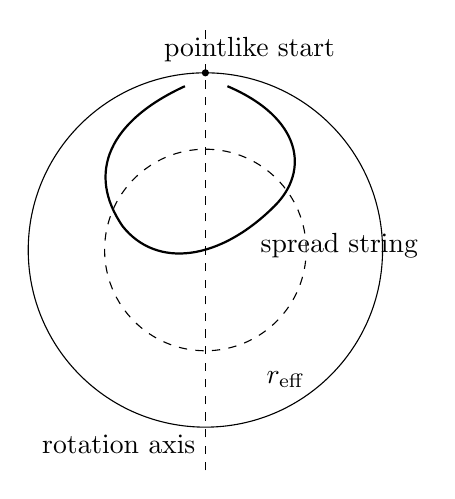
\begin{tikzpicture}[scale=1.0]
\draw (0,0) circle (2.25);
\draw[dashed] (0,-2.8) -- (0,2.8);
\draw[dashed] (0,0) circle (1.28);
\fill (0,2.25) circle (1.3pt);
\draw[thick]
(-0.26,2.08)
.. controls (-1.22,1.64) and (-1.52,0.98) .. (-1.05,0.30)
.. controls (-0.62,-0.24) and (0.18,-0.14) .. (0.88,0.56)
.. controls (1.33,1.01) and (1.22,1.68) .. (0.28,2.08);
\node at (0.56,2.55) {pointlike start};
\node at (1.70,0.05) {spread string};
\node at (-1.10,-2.47) {rotation axis};
\node at (1.02,-1.65) {$r_{\mathrm{eff}}$};
\end{tikzpicture}
\caption{Transcript-backed reconstruction of the north-pole picture: as more modes are included, the spread-out string behaves as though it were moving on a smaller effective sphere.}
\end{figure}

For a rotating extended object, the moment of inertia is obtained by integrating the mass distribution against the square of the distance to the axis. The key point is then immediate: once the string droops away from the north pole, some of its mass sits effectively closer to the rotation axis than the pointlike approximation assumed. For the purpose of this mechanical argument we keep the total mass fixed. Then the only thing that changes is the mass distribution, and therefore
\begin{equation}
I_{\mathrm{eff}}<mr^2.
\end{equation}
So the rotational energy behaves as if the string were a point particle on a sphere of smaller radius:
\begin{equation}
E\sim \frac{L^2}{2I_{\mathrm{eff}}}
=
\frac{L^2}{2m r_{\mathrm{eff}}^2},
\qquad
r_{\mathrm{eff}}<r.
\end{equation}

This is the beginning of the renormalization-group picture. Suppose we cut off the oscillator sum at some modest \(n_{\max}\). Then the string behaves like a somewhat fuzzy lump moving on a slightly smaller sphere. Now increase the cutoff and include still more short-distance structure. The same reasoning applies again, but now to that already reduced effective geometry. The result is another inward shift, and then another. The effective sphere keeps shrinking as more modes are restored.

\subsection{Question \& Answer}

\paragraph{Question.} Why do strings on spheres fail even though point particles do not?

\paragraph{Answer.} Because curvature couples the internal spread of the string back into the center-of-mass motion. A point particle has no internal extension, so the geometry enters only through a fixed moment of inertia. A string, by contrast, spreads out more and more as higher modes are included. On a curved background that spreading changes the effective moment of inertia, so the geometry seen by the string keeps changing with the cutoff. There is no stable limit.

This is the lecture's blunt conclusion: strings on spheres are not good theories. The problem is not merely that the string is large. The problem is that the effective geometry runs away.

\section{Effective Geometry, Ricci Flow, and the Einstein Equations}

The sphere has now done its job. It has taught us what kind of failure to look for in a general background. From this point on, the right variable is not the shape of one particular sphere but the metric itself. A geometry is described by its metric tensor \(g_{\mu\nu}(x)\), and the question becomes: how does the \emph{effective} metric seen by the spread-out string change as the cutoff changes?

\begin{figure}[h]
\centering

\includegraphics[width=0.72\textwidth]{lecture_09_figure_03.png}
\caption{Metric tensor notation on the board.}
\end{figure}

The image preserves the moment at which the metric is introduced on the board. It does not, by itself, fix the full equation, since the right-hand side is cut off and the left board still contains earlier material. The lecture, however, makes the logic very clear. The change in the metric is a symmetric rank-two tensor. It must vanish when the background is flat. Therefore the right-hand side must be built from curvature and must itself be a symmetric rank-two tensor. The natural candidate is the Ricci tensor \(R_{\mu\nu}\), obtained by contracting the full curvature tensor.

Thus the cutoff dependence takes the schematic form
\begin{equation}
\delta g_{\mu\nu}(x)\propto -\,R_{\mu\nu}(x),
\end{equation}
or, in the logarithmic language used in the lecture,
\begin{equation}
\frac{d g_{\mu\nu}}{d\log \Lambda}\propto -\,R_{\mu\nu}.
\end{equation}
The sign is fixed heuristically by the sphere example: positive curvature makes the effective sphere shrink, so the flow must point inward.

\subsection{Question \& Answer}

\paragraph{Question.} What must the geometry do if string theory is to have a sensible limit on it?

\paragraph{Answer.} The effective geometry must stop running as the cutoff is raised. In other words, the metric must approach a fixed point of the flow. At leading order that means precisely that the Ricci tensor vanishes:
\begin{equation}
R_{\mu\nu}=0.
\end{equation}

\begin{definition}
A geometry satisfying \(R_{\mu\nu}=0\) is called \emph{Ricci flat}. In the present lecture, Ricci flatness is the condition that the string background be stable under the addition of ever shorter-distance modes.
\end{definition}

Susskind then turns this into the major payoff of the lecture. Ricci flatness is not only the fixed-point condition for the string. It is also the vacuum Einstein equation. The board displays the Einstein tensor in the usual form:

\begin{figure}[h]
\centering

\includegraphics[width=0.80\textwidth]{lecture_09_figure_04.png}
\caption{Einstein tensor written in terms of curvature and stress tensor.}
\end{figure}

\begin{equation}
G_{\mu\nu}=R_{\mu\nu}-\frac{1}{2}g_{\mu\nu}R=T_{\mu\nu}.
\end{equation}
In empty space,
\begin{equation}
T_{\mu\nu}=0,
\end{equation}
so the field equation becomes
\begin{equation}
G_{\mu\nu}=0.
\end{equation}
Taking the trace yields
\begin{equation}
g^{\mu\nu}G_{\mu\nu}
=
R-\frac{D}{2}R
=
0,
\end{equation}
and therefore, in the dimensions relevant here,
\begin{equation}
R=0.
\end{equation}
Substituting back into the vacuum equation gives
\begin{equation}
R_{\mu\nu}=0.
\end{equation}

So the consistency condition for string propagation reproduces the vacuum Einstein equations. That is the first promise of the lecture fulfilled: gravity appears because a string can propagate consistently only on backgrounds that solve Einstein's equations.

A second remark is inserted at exactly this point in the lecture's rhythm. Ricci flatness is not by itself the entire story. The cutoff independence works only in the critical dimension: \(10\) for the superstring and \(26\) for the bosonic string. The lecture mentions this as a caveat rather than reopening the derivation, and that is the right balance here as well.

\section{Compactification and Toroidal Backgrounds}

Only after the gravity result is in place does the lecture turn to the practical question: what do we do with \(10\) or \(26\) dimensions? The answer is compactification. We do not remove the extra dimensions; we roll them up so that ordinary coarse-grained probes do not see them as large directions of motion.

The lecture insists, sensibly, that these extra dimensions are taken to be spatial. More than one time direction is set aside, not because every conceivable theory with multiple times has been ruled out in advance, but because the simple quantum theories we know how to formulate do not make sense that way. Compact spatial directions, by contrast, give concrete and solvable models.

Susskind introduces compactification in the most elementary possible way. Imagine a world that looks one-dimensional at large scales: a line on which particles move back and forth. Now imagine that, under a microscope, the line is discovered to be the surface of a cylinder. Large objects do not notice the circular direction, but small objects can move both along the line and around the circle. That is the basic picture of a hidden dimension.

To make this mathematically clean we describe the cylinder as a ribbon with its two horizontal edges identified. One exits through one edge and re-enters through the opposite edge. There is then no genuine boundary. The same trick may be repeated with more than one pair of identified faces, producing higher-dimensional tori.

\begin{figure}[h]
\centering
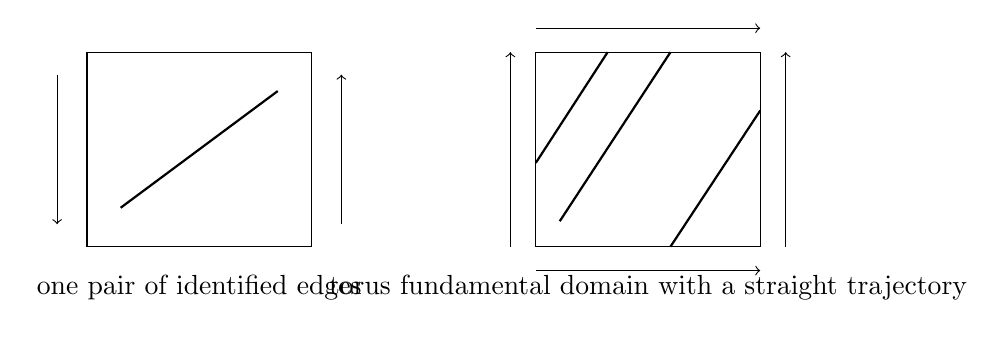
\begin{tikzpicture}[scale=0.95]
\draw (-6,-1.3) rectangle (-3,1.3);
\draw[->] (-6.4,1.0) -- (-6.4,-1.0);
\draw[->] (-2.6,-1.0) -- (-2.6,1.0);
\draw[thick] (-5.55,-0.78) -- (-3.45,0.78);
\node at (-4.5,-1.85) {one pair of identified edges};

\draw (0,-1.3) rectangle (3,1.3);
\draw[->] (0,1.62) -- (3,1.62);
\draw[->] (0,-1.62) -- (3,-1.62);
\draw[->] (-0.34,-1.3) -- (-0.34,1.3);
\draw[->] (3.34,-1.3) -- (3.34,1.3);
\draw[thick] (0.32,-0.96) -- (1.80,1.3);
\draw[thick] (1.80,-1.3) -- (3.0,0.52);
\draw[thick] (0.0,-0.18) -- (0.96,1.3);
\node at (1.5,-1.85) {torus fundamental domain with a straight trajectory};
\end{tikzpicture}
\caption{Transcript-backed reconstruction of periodic identification: first a cylinder, then a torus presented as a rectangle with opposite sides identified.}
\end{figure}

This now leads directly into the lecture's insistence that a torus is, first of all, a topology. We must not think primarily of the curved bagel embedded in \(\mathbb{R}^3\). For compactification what matters is the identified flat fundamental domain. A torus may be cut open into a cylinder, and then cut again into a rectangle. The rectangle is not a different object; it is the same torus presented with identifications remembered.

This way of presenting the torus also makes clear why it is the simplest useful compact space in string theory. The flat fundamental domain has zero curvature. In particular it is Ricci flat. Hence it satisfies exactly the condition that emerged from the first half of the lecture.

The lecture then asks how many inequivalent flat tori there are. At the level needed here, there are three continuous parameters: an overall size, an aspect ratio, and a shear or twist before the opposite sides are identified. Turning the rectangle on its side does not produce a new torus, so the aspect ratio is counted only up to that trivial equivalence.

\begin{figure}[h]
\centering
\begin{tikzpicture}[scale=1.0]
\draw (0,0) rectangle (3,2);
\draw[<->] (0,-0.35) -- (3,-0.35);
\draw[<->] (-0.35,0) -- (-0.35,2);
\node at (1.5,-0.7) {width};
\node[rotate=90] at (-0.75,1.0) {height};

\draw (5,0) -- (8,0) -- (8.9,2) -- (5.9,2) -- cycle;
\draw[dashed] (5,0) -- (5.9,2);
\draw[<->] (5.0,2.35) -- (5.9,2.35);
\node at (6.85,2.7) {twist};
\end{tikzpicture}
\caption{A flat torus described by its fundamental domain: overall size, aspect ratio, and twist. The lecture uses the names K\"ahler modulus, complex-structure modulus, and Dehn twist in an explanatory but not fully formal sense.}
\end{figure}

The lecture briefly mentions more complicated Ricci-flat compactifications, especially Calabi--Yau manifolds, but only as a glance toward the larger subject. The conceptual point has already been made: tori are the easiest compact Ricci-flat backgrounds, and therefore the easiest place to see string theory working consistently in extra dimensions.

\section{Circle Compactification, Winding States, and T-Duality}

The last step is to focus on the simplest compactification of all: one compact circle. From here on we denote its radius by \(R\), reserving the earlier \(r\) for the sphere. What becomes observable in lower dimensions is not the compact direction itself but the spectrum associated with motion and winding around it.

The lecture first writes the massless energy-momentum relation on the board:

\begin{figure}[h]
\centering

\includegraphics[width=0.72\textwidth]{lecture_09_figure_05.png}
\caption{Massless energy as the magnitude of momentum.}
\end{figure}

\begin{equation}
E=c|P|.
\end{equation}
The important visual point in the board image is the absolute value: the sign of a momentum component may change, but the energy is positive. Later in this discussion the lecture effectively sets \(c=\hbar=1\).

Now suppose the compact circle has circumference \(2\pi R\). Momentum around that circle is quantized for the same reason angular momentum is quantized:
\begin{equation}
p_cR=n\hbar.
\end{equation}
Setting \(\hbar=1\) gives
\begin{equation}
p_c=\frac{n}{R}, \qquad n\in\mathbb{Z}.
\end{equation}
If the particle is massless in the full higher-dimensional theory and carries no momentum in the noncompact directions, then from the lower-dimensional point of view its energy is entirely the energy of motion around the circle. That energy is therefore interpreted as mass:
\begin{equation}
m_n=\frac{|n|}{R}.
\end{equation}
This is the Kaluza--Klein tower. The smaller the circle, the larger the spacing between these masses.

String theory now introduces something genuinely new. A closed string can wrap around the compact circle. If we set the string tension to \(1\), as the lecture does for simplicity, then the energy of a wound string is proportional to its length, hence to the radius of the circle. A string wound \(w\) times therefore has mass
\begin{equation}
m_w=|w|R,
\qquad
w\in\mathbb{Z}.
\end{equation}
Again the absolute value matters. Positive and negative winding correspond to opposite orientations, not to negative mass.

So the compact circle gives two towers of states,
\begin{align}
m_n &= \frac{|n|}{R},\\
m_w &= |w|R.
\end{align}
They are complementary. When \(R\) is small, the momentum tower is widely spaced and the winding tower is closely spaced. When \(R\) is large, the situation is reversed.

\begin{figure}[h]
\centering
\begin{tikzpicture}[scale=0.96]
\draw[->] (0,0) -- (0,4.6);
\foreach \y/\lab in {0/0,1.2/{1/R},2.4/{2/R},3.6/{3/R}}
{
\draw (-0.16,\y) -- (0.16,\y);
\node[left] at (-0.2,\y) {$\lab$};
}
\node at (0,-0.55) {Kaluza--Klein};

\draw[->] (5,0) -- (5,4.6);
\foreach \y/\lab in {0/0,1.2/{R},2.4/{2R},3.6/{3R}}
{
\draw (4.84,\y) -- (5.16,\y);
\node[right] at (5.2,\y) {$\lab$};
}
\node at (5,-0.55) {winding};
\end{tikzpicture}
\caption{Transcript-backed mass ladders for momentum modes and winding modes. The exchange \(R\leftrightarrow 1/R\) swaps the two towers.}
\end{figure}

\subsection{Question \& Answer}

\paragraph{Question.} Can winding states be absent if we start without them?

\paragraph{Answer.} No, not in a theory of closed strings. The lecture answers this dynamically. Start with a closed string of zero net winding. Stretch it around the compact direction so that one segment effectively winds one way and another segment winds the other way. The total winding is still zero. But the basic closed-string interaction is rearrangement: one connected string can reconnect into two disconnected closed strings. After the rearrangement one obtains two particles with opposite winding numbers. Send one far away and, locally, a winding state remains. So winding states are not optional sectors one may simply forbid; the dynamics produces them.

With both towers present, the final surprise is unavoidable. If we exchange
\begin{equation}
R \longleftrightarrow \frac{1}{R},
\qquad
n \longleftrightarrow w,
\end{equation}
the two spectra are interchanged. In particular the set of masses is unchanged. At the special point \(R=1\) in these units, the two towers coincide exactly. If we try to shrink the circle past this scale, the theory does not continue to produce genuinely new physics. It reorganizes itself into the description of a larger circle.

That is T-duality. The lecture is careful here as well. The equality of the simple spectra is only the first hint. The stronger claim is that, for closed strings, the entire theory is symmetric under this exchange: not only the masses, but the full spectrum and the scattering amplitudes. This is not a property of point-particle mechanics on a compact circle. It is a specifically stringy fact because only strings possess both momentum and winding sectors.

The closing philosophical point is just as important as the formulas. Geometry can often be read from a spectrum, just as one learns something about a drum from its vibrational frequencies. But string theory also teaches us that the spectrum need not determine geometry uniquely. Two geometries that look very different to point-particle intuition can be the same background for strings.

\section{Summary}

The lecture opens with a consistency question and turns it into gravity. A point particle on a smooth curved space has a sensible continuum limit. A string need not. On a sphere the zero-point spreading of the string changes the effective moment of inertia, and as more modes are added the effective geometry keeps running inward. The correct general language is then a flow of the metric,
\[
\delta g_{\mu\nu}\propto -R_{\mu\nu},
\]
and the condition for stability is Ricci flatness. But \(R_{\mu\nu}=0\) is precisely the vacuum Einstein equation. In this way, gravity appears as a consistency condition for string propagation.

Only after that does the lecture turn to extra dimensions. The simplest way to hide them is toroidal compactification, where the compact directions are periodically identified and the resulting flat tori are automatically Ricci flat. On a compact circle the spectrum contains both Kaluza--Klein momentum modes with masses proportional to \(1/R\) and winding modes with masses proportional to \(R\). Their exchange under \(R\leftrightarrow 1/R\) is T-duality. The final lesson is then twofold: consistency selects the geometry, and the spectrum of strings reshapes what we even mean by geometry in the first place.